\documentclass[UTF8]{ctexbook}

% SCI book 的模板 sty,适用于中文
\usepackage{scibookchn}
\usepackage{scigeneral}

\title{王新龙声学博文}

% start each section on a new page
\let\stdsection\section
\renewcommand\section{\newpage\stdsection}


\begin{document}

\maketitle

\tableofcontents

\chapter{声波的基本性质}
\section{流体力学引论}

\emph{摘要}\ 流体之声是流体质点振动形式和能量的传递。
所以,声学与流体动力学存在某种程度的相关性。
欲精通声学理论,必先掌握必要的流体力学基本知识和基本理论。
无奈在教学实践中发现,仍有不少学生阙如,一定程序上影响了《声学基础》课的
学习进程。
监于此,本文简介理想流体的流体力学基本理论,以期作为读者钻研声学的预备。

\emph{正文}\ 流体包括气体和液体,可流动而固定形状(除非置于固定形状的容器之内)。
尽管流体由微观上离散的分子或原子组成,但流体力学仅研究流体的宏观力学现象。
所以,流体力学把流体视若宏观连续的媒质。
流体力学的理论分析涉及到流体的「体积元」概念。
所谓体积元,概指宏观无限小但微观可包含大量流体分子(或原子)者。
宏观无限小意谓体积元内宏观物理量几乎是均匀,因此可描述体积元所在空间的「点」
的流体状态。
另一方面,这些物理量必须具有统计物理的意义,因此微观上必须足够大,以包含
大量分子(或原子),也即,体积元的尺寸必须远大于分子的平均自由程。
\emph{体积元是纯空间概念},与之相关但相异的概念是流体的「质点」。
所谓质点(particle),其实也是如此这般的流体体积元,但\emph{
	质点是流体的微实体,
具有质量},可视为流体的宏观「分子」(犹如可变形的流体微粒)。
无数质点的运动遂构成了流体的运动。

\section{声学量的复数运算\\
Complex Operations for Acoustical Quantities}

\emph{摘要}\ 振动与声学量虽然是可观测的实数物理量,但也可用复数表示。
复数表示不但可极大地简化数学演算,因此无论在线性还是非线性的声学理论中均
广泛采用复数表示声学量。本文简述声学量的复数表示及运算规则,并举例说明。

设小写的$x$为实数量,而大写的$X$为对应的复数量,即$x=\Re(X)$,其中
$\Re(X)$表示取复数量$X$的实部,即
$$
x = \Re(X) = \frac12(X+X^*)
$$
其中右上标的星号「*」表示复共轭操作。显然,实数量$x$与其对应的复数量$X$并非
一一对应。复数量$X$加上任意的线虚数$\mj y$并不影响其意义:
$$
x = \Re(X) = \Re(X+\mj y)
$$

\subsection{加法规则}
若$x$、$y$和$z$为实数量,$a$和$b$是任意的实数,$z=ax+by$。设$x$、$y$和$z$
对应的复数量分别为$X$、$Y$和$Z$,即$x=\Re(X)$、$y=\Re(Y)$和$z=\Re(Z)$,则
因
$$
z = ax+by = \Re(aX+bY) = \Re(Z)
$$
所以,复数量$X$、$Y$和$Z$之间存在以下关系
$$Z=aX+bY$$
现设$x$是时间$t$的函数:$x=x(t)$。它对应的复数量$X$也是时间的函数:$X=
X(t)$。由于导数和积分本质上是线性加法去处,因此存在关系:
$$\dv{t} \Re(X) =\Re\qty(\dv{X}{t})\qc \int \Re(X) \dd{t} = \Re 
\qty(\int X\dd{t})$$

即复数$\dv*{X}{t}$是实数量导数$\dv*{x}{t}$对应的复数量,复数积分$\int X
\dd{t}$是实数积分$\int x\dd{t}$对应的复数量。

\subsection{乘法规则}
现设$z$是$x$和$y$之积,$z=xy$,对应的复数量为$Z$。根据定义,
$$z=xy =\Re(X)\Re(Y) = \Re(\Re(X)Y)=\Re(X\Re(Y))$$
所以,
\begin{subequations}
	\label{eq:complexop_Z}
	\begin{equation}Z= \Re(X)Y = \frac12 (XY+X^*Y)\end{equation}
	\begin{equation}Z=X\Re(Y) = \frac12 (XY+XY^*)\end{equation}
\end{subequations}
再次申明,式(\ref{eq:complexop_Z})中两个表式所给出的$Z$在数学上严格而言是
不等的,只因$Z$的实部才有物理意义,故两种表示在物理上等价。

\subsection{时间简谐量的周期平均值}
复数表示对于简谐声学量的计算尤其有效。假设与时间$t$的依赖关系为$\exp(\mj 
\omega t)$,其中$\omega = 2\uppi /T$为频率,$T$是振动周期,$\mj$是虚数单位
。例如,$X$和$Y$是时间简谐的复量
$$X=X\st{a} \me^{\mj \omega t }\qc Y = Y\st{a}\me^{\mj \omega t}$$
其中,$X\st{a}$和$Y\st{a}$分别为$X$和$Y$的复振幅,是与时间$t$无关的常数。
则有
$$\dd{X}{t}=\mj \omega X\qc \int X\dd{t} = \frac{X}{\mj \omega}$$
根据(\ref{eq:complexop_Z}),此时乘积$z=xy$的复数表达式为
$$Z=\frac12 X\st{a}^* Y\st{a}+\frac12 X\st{a}Y\st{a}\me^{2\mj \omega t}$$
上式第二项有时间依赖关系$\exp(2\mj \omega  t)$,描述了乘积量$z$的瞬态运动。
这是一个二次谐波(频率$2\omega$),其周期平均为零。第一项是与时间无关的
「直流」项,等于复量$Z$的周期平均值:
$$\bar{Z} = \frac1T \int_0^T Z(t) \dd{t} = \frac12 X\st{a}^* Y\st{a} =
\frac12 X^* Y$$
所以,乘积量$z=xy$的周期均值为
$$\bar{z}=\frac1T \int_0^T z\dd{t} = \overline{\Re(Z)} = \Re(\bar{Z})
=\frac12\Re(X^*Y)$$
即,存在以下重要的乘积平均法则
\begin{equation}
	\overline{x(t)y(t)} = \frac12 \Re(X^*Y) \label{eq:complexop_xy}
\end{equation}
对于简谐振动而言,振动物理量本身的时间均值往往为零。但如振动量的乘积等非
线性运算,多产生类似的「直流」项,因而平均值非零。\emph{「直流」和高次谐波
的产生为典型的非线性效应。}

以下以若干典型振动与声学量为例,说明复数运算的应用。

\subsubsection{单振子周期平均能量}
设有质量为$M\st{m}$、弹性系数为$K\st{m}$的单振子,其质点的位移为$x$,速度
$v$,对应的复位移为$X$,复速度为$V$。单振子的势能和动能分别为
$$E\st{p} = \frac12 K\st{m} x^2 = \frac12 K\st{m}\qty[\Re(X)]^2$$
$$E\st{k} = \frac12 M\st{m} v^2 = \frac12 M\st{m} \qty[\Re(V)]^2$$
若单振子仅作简谐振动,则根据式(\ref{eq:complexop_xy}),势能和动能的一个周期
平均值分别为
$$\overline{E\st{p}} = \frac12 K\st{m} \overline{x^2} = \frac14 K\st{m}
|X|^2$$
$$\overline{E\st{k}} = \frac12 M\st{m} \overline{v^2} = \frac14 M\st{m}
|V|^2$$
对于自由振动,
$$V = \mj \omega_0 X\qc \qty(\omega_0 = \sqrt{\frac{K\st{m}}{M\st{m}}})$$
代入前式,知平均势能等于平均动能:
$$\overline{E\st{p}} = \overline{E\st{k}}$$

\subsubsection{声能通量密度和声强的运算}
声能通量密度$\vb{I}$为声压$p$与速度适量$\vb{v}$的乘积:$\vb{I}=p \vb{v}$。
声压、速度和声能通量密度等物理量本身是实量,但均可以用复数表示。在振动
与声的问题中,极大部分情形下所涉及的是复数量及其运算,因此在下文中我们放弃
前面用大写字母表示复量的做法,而一概约定:除非特别说明,\emph{所有的变量符号
均表示对应实量的复量},如声压、复速度和复能量通量密度仍用$p$、$\vb{v}$和
$\vb{I}$表示;如果确实需要用到实数量,则只要对这些复数量取实部操作$\Re$即可
。例如,根据公式(\ref{eq:complexop_Z}),复声能通量密度的公式可写成
\begin{equation}
	\label{eq:complexop_I}
	\vb{I} = \frac12 p\vb{v} + \frac12 p^* \vb{v}
\end{equation}
取实部$\Re(\vb{I})$即为实声能通量密度。

对频率为$\omega$的简谐声波,公式(\ref{eq:complexop_I})的第一项描述声能通量
密度之瞬变,而第二项是「直流」分量,为复声能通量密度之时间均值:
\begin{equation}
	\label{eq:complexop_barI}
	\overline{\vb{I}} = \frac1T \int_t^{t+T}\dd{t} = \frac12 p^* \vb{v}
\end{equation}
取其实部即得到\emph{声强}:
$$\Re(\overline{\vb{I}}) = \frac12 \Re\qty(p^* \vb{v})$$
可见,采用复运算,易分离场量(此处是声能通量密度)的时变和时不变成份。

对于平面行波,传播方向为$\vb{n}$(单位矢量),则媒质质点的振速$\vb{v}
=(p/z_0)\vb{n}$,代入公式(\ref{eq:complexop_I})和(\ref{eq:complexop_barI})
得到
$$\vb{I} = \frac{1}{2z_0}\qty(p^2+|p|^2)\vb{n}$$
$$\overline{\vb{I}} = \frac{1}{2z_0} \overline{\qty(p^2+|p|^2)}
=\frac{|p|^2}{2\rho_0 c_0 }\vb{n}$$
式中$z_0=\rho_0c_0$是媒质的声特性阻抗率。

\subsubsection{声能密度复数运算}
对平面波而言\footnote{编著添加。},用实声学量表示的流体声场的(瞬时)声能
密度为
$$\eps = \frac12 \rho_0 \qty[\vb{v} \vdot \vb{v} +\qty(\frac{p}{z_0})]$$
其中的声压$p$和速度$\vb{v}$是实数量。若全改用复量表示,且仍采用相同的变量
符号,则上式应改为
\begin{align}
	\label{eq:complexop_eps}
	\eps & = \frac14 \rho_0 \qty[(\vb{v}\vdot\vb{v} + \vb{v}^*\vdot
	\vb{v}) +\frac{1}{z_0^2} \qty(p^2+p^* p)]\nonumber\\
	& = \frac14 \rho_0 \qty[\vb{v}\vdot\vb{v}+ \qty(\frac{p}{z_0} )^2]
	+\frac14 \rho_0 \qty(\vb{v}^*\vdot \vb{v} + \qty|\frac{p}{z_0}|^2)
\end{align}
对频率$\omega$的简谐声波,公式(\ref{eq:complexop_eps})后一等式中的第一项描述
声能密度的瞬时变化,而第二项是「直流」分量,为复声能密度之时间周期平均值,
取其实部即为平均声能密度。因此,简谐声场的平均声能密度为
\begin{equation}
	\label{eq:complexop_bareps}
	\overline{\eps} = \frac14 \rho_0 \qty(|\vb{v}|^2 +\frac{|p|^2}{z_0^2})
\end{equation}

对于沿方向$\vb{n}$传播的平面行波,把$\vb{v}=(p/z_0)\vb{n}$代入公式
(\ref{eq:complexop_eps})和(\ref{eq:complexop_bareps})得到
\begin{align*}
	\eps &= \frac{1}{2\rho_0c_0^2} (p^2+|p|^2)\\
	\overline{\eps} &= \frac{1}{2\rho_0c_0^2} |p|^2
\end{align*}


\section{全反射状态的声场与声能流}
英文标题:
Sound Fields and Energy Flux Under Total Reflection

Web:
http://xlwangnu.blog.163.com/blog/static/190719270201192502043374/

\emph{摘要}
全反射是常见声光现象。在媒质交界面上,若入射媒质的声速不如透射媒质的(或折
射率小于1),则当入射角足够大就会发生全反射,入射声能悉数反射。虽然如此,
全反射下声场如何分布?透射媒质中是否存在声场?如存在,取何种波动方式?此
正本文试图回答的问题。分析表明,在全反射下,(1)入射媒质中的总声场在界面法
向呈驻波形式,而在界面切向呈行波形式;(2)仍存在透射声波,但以沿界面传播的
表面波形式存在,但垂直于界面的方向上指数衰减。

若透射媒质的声速$c_2$大于入射媒质的声速$c_1$,且入射角(incident angle)
$\theta\st{i}$大于全反射临界角$\theta\st{ic}$,
\begin{equation}
\theta\st{ic} = \arcsin \frac{c_1}{c_2} = \arcsin n, \qty(n=\frac{c_1}{c_2}
<1)
\end{equation}
声波全部反射。此即著名的\emph{声全反射现象}(total reflection)。与光
的全反射略有不同,声的全反射一般发生在“硬界面”,如从空气到水,从水到固体。
光的全反射则发生在“软表面”---从光密介质入射到光疏介质,如光纤内的光反射,故
而一般称之为全内反射(Total internal reflection)。或问:在全反射状态,声场
分布如何?声能如何传播?此正本文所欲讨论的。

\subsection{声场分布}
如图xx所示,频率为$\omega$的平面声波从声特性阻抗率为$\rho_1c_1$的媒质中以角
度$\theta\st{i}$入射到声特性阻抗率为$\rho_2c_2$的媒质上。
设入射方向和两媒质边界面的法向构成的平面为$(x,y)$平面,$x$轴沿边界内法向,
$y$轴在边界平面上。根据平面行波论,入射(incident)、反射(reflected)和
透射(transmitted)的声场解各具如下形式:
\begin{equation}
	\label{eq:totalref_pressure}
	\begin{cases}
	p\st{i} = p\st{ia} \me^{-\mj k_1 \vb{n}\st{i} \vdot \vb{r}}
	\qc \vb{v}\st{i} = \dfrac{p\st{i}}{\rho_1c_1} \vb{n}\st{i}\\
	p\st{r} = p\st{ra} \me^{-\mj k_1 \vb{n}\st{r} \vdot \vb{r}}
	\qc \vb{v}\st{r} = \dfrac{p\st{r}}{\rho_1c_1} \vb{n}\st{r}
	\qc (p\st{ra} = r_p p\st{ia}) \\
	p\st{t} = p\st{ta} \me^{-\mj k_2 \vb{n}\st{t} \vdot \vb{t}}
	\qc \vb{v}\st{t} = \dfrac{p\st{t}}{\rho_2c_2} \vb{n}\st{t}
	\qc (p\st{ta} = t_p p\st{ta}) 
	\end{cases}
\end{equation}
式中,$p\st{ia}$、$p\st{ra}$和$p\st{ta}$分别为入射、反射和透射(折射)
波的声压幅度,$r_p$和$t_p$分别为声压反射系数和透射系数,$\theta\st{t}$为
折射角(refracted angle),$k_1$和$k_2$分别为入射和透射媒质的波数,
而$\vb{n}\st{i}$、$\vb{n}\st{r}$和$\vb{n}\st{t}$则依次为入射、反射和
折射波的方向矢量,
\begin{equation}
	\label{eq:totalref_n}
	\vb{n}\st{i}=(\cos \theta\st{i}, \sin \theta\st{i})\qc 
	\vb{n}\st{r}=(-\cos \theta\st{r}, \sin \theta\st{r})\qc 
	\vb{n}\st{t}=(\cos \theta\st{t}, \sin \theta\st{t})
\end{equation}
在$\vb{n}\st{r}$表达式中,已利用了关系$\vb{theta}\st{r}=\theta\st{i}$。为
简洁起见,本文一根省略时间因子$\exp(\mj \omega t)$。

根据Snell定律(折射律),
\begin{equation}
	\label{eq:totalref_snell}
	\sin\theta\st{t} = \frac{\sin\theta\st{i}}{n}\qc (n<1)
\end{equation}
当$\theta>\theta\st{ic}$时,$\sin\theta\st{t}>1$,$\theta\st{t}$不复为实数
而是复数。是以,作复变换:$\theta\st{t} \rightarrow \psi$,
\begin{equation}
	\label{eq:totalref_theta_trans}
	\theta\st{t} = \frac{\uppi}{2}+\mj \psi\qc 
	\begin{cases}
		\sin \theta\st{t} = \cosh \psi\\
		\cos\theta\st{t} = -\mj \sinh \psi
	\end{cases}
\end{equation}
代入折射公式(\ref{eq:totalref_snell}),则 Snell定律改为
\begin{equation}
	\label{eq:totalref_snell2}
	\cosh \psi = \frac{\sin \theta\st{i}}{n}
\end{equation}
由此可知,$\psi$具有实数解。当$\theta\st{i}$从$\theta\st{ic}$增至$\uppi/2$
时,$\psi$从$0$单调增大至$\arccosh(1/n)>0$。此处杂提醒读者,数学上,变换
(\ref{eq:totalref_theta_trans})中的$\psi$可正可负。但考虑到下面公式xx(12)
给出的透射声压解$p\st{t}$中,声波必沿$x$正向衰减,$\psi$只能取正值。引入变
换(\ref{eq:totalref_theta_trans})后,全反射($\theta\st{i}>\theta\st{ic}$)
状态下的声压反射系数$r_p$和透射系数$t_p$可表为\footnote{编者著:利用$x=0$
处的边界条件,即$\begin{cases}1+r_p = t_p\\ \dfrac{1-r_p}{z\st{s1}} =
	\dfrac{t_p}{z\st{s2}}\end{cases}$,其中法向声阻抗率分别是
$z\st{s1}= \rho_1c_1/\cos \theta\st{i}, z\st{s2} = \rho_2c_2
/\cos\theta\st{i}$,得到$r_p = \dfrac{z\st{s2}-z\st{s1}}{z\st{s2}+z\st{s1}}
$。}
\begin{equation}
	\label{eq:totalref_rptp}
	\begin{cases}
		r_p & = \dfrac{p\st{ra}}{p\st{ia}} = \dfrac{m\cos \theta \st{i} +
	\mj n \sinh \psi }{m\cos \theta\st{i} - \mj n \sinh \psi} = 
	\me^{2\mj \phi}\\
	t_p&=\dfrac{p\st{ta}}{p\st{ia}} = \dfrac{2m\cos \theta \st{i}}{m\cos 
		\theta\st{i} - \mj n \sinh \psi} = 2\cos\phi \me^{\mj \phi}
	\end{cases}
	\qc \qty(m = \frac{\rho_2}{\rho_1})
\end{equation}
式中的相位角$\phi$由下列公式给出
\begin{equation}
	\tan \phi = \frac{n\sinh \psi}{m \cos \theta\st{i}} = 
	\frac{\rho_1c_1}{\rho_2c_2} \frac{\sinh \psi}{\cos \theta\st{i}}
	\qc \qty(0<\phi<\frac{\uppi}{2})
\end{equation}
从式(\ref{eq:totalref_rptp})可见,当入射角$\theta\st{i}$大于临界角
$\theta\st{ic}$时,反射波的振幅等于入射的($|r_p|=1$),但入射和反射
声压间存在$2\phi$的相位差。把$r_p=\exp(2\mj \phi)$代入入射和反射声压表达
式(\ref{eq:totalref_pressure}),两者相加再简化,得到入射侧的总声压场
$p_1$和速度场$\vb{v}_1=(v_{1,x}, v_{2,y})$的表达式
\begin{equation}
	\label{eq:totalref_pv1}
	\begin{cases}
		p_1&= p\st{i}+p\st{r} = 2p\st{ia}\cos(k_1x\cos\theta\st{i}+\phi)
		\me^{-\mj (k_1y\sin\theta\st{i}-\phi)}\\
		v_{1,x}&= v_{\mi x} + v_{\mathrm{r}x} = 2v\st{ia}\sin
		(k_1x\cos\theta\st{i}+\phi)\cos\theta\st{i}
		\me^{-\mj \qty(k_1y\sin\theta\st{i}-\phi+ \uppi/2)}\\
		v_{1,y}&= v_{\mi y} + v_{\mathrm{r}y} = 2v\st{ia}\cos
		(k_1x\cos\theta\st{i}+\phi)\sin\theta\st{i}
		\me^{-\mj \qty(k_1y\sin\theta\st{i}-\phi)}
	\end{cases}
	\qc \qty(v\st{ia} = \frac{p\st{ia}}{\rho_1c_1})
\end{equation}
式中,$v\st{ia}$是入射声波质点速度振幅。可见,入射侧声场因全反射而在法向
(负$x$方向)形成了驻波,但沿界面($y$方向)仍是传播的。沿界面的传播的相速度和波长分别为
\begin{equation}
	\label{eq:totalref_interface1}
	\begin{cases}
		c_{1y} & = \dfrac{\omega}{k_1\sin \theta\st{i}}
		=\dfrac{c_1}{\sin\theta\st{i}} \geq c_1\\
		\displaystyle
		\lambda_{1y} &= \dfrac{2\uppi}{k_1\sin\theta\st{i}}
		=\dfrac{\lambda_1}{\sin\theta\st{i}} \geq\lambda_1
	\end{cases}
\end{equation}
所以,沿界面传播的相速度大于入射媒质的常规声速$c_1=\omega /k_1$,波长$\lambda
_{1y}$比常规波长$\lambda_1 = k_1/2\uppi$要长;仅当入射波完全平行于界面
($\theta\st{i}=\uppi/2$)时,$c_{1y}=c_1$,$\lambda_{1y}=\lambda_1$。
公式(\ref{eq:totalref_pv1})也表明,在全反射下,法向驻波声场依赖于入射角
$\theta\st{i}$的相位$\phi$,故驻波的波节和波腹位置因入射角$\theta\st{i}$
变化而发生漂移。值得注意的是,在临界全反射($\theta\st{i}=\theta\st{ic}$)下,
$\phi=0$,$t_p=2$,即透射声压是入射声压的两倍。当入射角$\theta\st{i}\to 
\uppi/2$(最大入射角)时,相位$\phi: 0\to \uppi/2$,透射系数的幅值$|t_p|$
从2降至0.从式(\ref{eq:totalref_pv1})还可看出,在入射侧的任意位置,速度分量
相位相差$\uppi/2$,流体质点在$(x,y)$平面上围绕平衡位置作椭圆运动,与单纯的
行波场不同。

把变换式(\ref{eq:totalref_snell})代入式(\ref{eq:totalref_n})中$\vb{n}\st{t}$
的表达式中,结果为:
\begin{equation}
\vb{n}\st{t} = (-\mj \sinh \psi, \cosh\psi)
\label{eq:totalref_nt}
\end{equation}
即透射波矢$\vb{k}\st{t} = k_2\vb{n}\st{t}$的法向分量是虚数,表明透射波在$x$
方向是非传播的。利用式(\ref{eq:totalref_rptp})给出的透射系数$t_p$和式
(\ref{eq:totalref_nt}),式(\ref{eq:totalref_pressure})中的透射声压$p\st{t}$
和速度矢量$\vb{v}\st{t}=(v_{\mathrm{t,} x}, v_{\mathrm{t,} y})$经整理可进一步表为
\begin{equation}
	\label{eq:totalref_pvt}
	\begin{cases}
		p\st{t} = 2p\st{ia} \cos \phi \me^{-k_2x\sinh \psi - \mj (k_2 y
		\cosh \psi -\phi)}\\
		v_{\mathrm{t,}x} = \dfrac{\rho_1c_1}{\rho_2c_2} 2v\st{ia} \cos\phi
		\sinh \psi \me^{k_2x\sinh \psi - \mj\qty(k_2y\cosh \psi -\phi
		+\uppi/2)}\\
		v_{\mathrm{t,}y} = \dfrac{\rho_1c_1}{\rho_2c_2} 2v\st{ia} \cos\phi
		\cosh \psi \me^{k_2x\sinh \psi - \mj\qty(k_2y\cosh \psi -\phi
		)}
	\end{cases}
\end{equation}
这表明,在全反射下透射波是沿界面传播、但法向衰减的\emph{声表面波}(surface
waves) --- 仅存在于边界面附近的声波,类似于固体表面的瑞利波(Rayleigh waves)
。透射波的幅度随离边界之深度$x$而指数衰减,若令$k_2x\sinh \psi = 1$,则得到
表面波的「透射深度」$x=d$为:
\begin{equation}
	2\uppi \frac{d}{\lambda_2} = \frac{1}{\sinh\psi} = \frac{n}{\sqrt{
		\sin^2\theta\st{i}-n^2}}
\end{equation}
所以,透射深度$d$是入射角$\theta\st{i}$的函数。当入射角$\theta\st{i}$大于
但接近临界角$\theta\st{ic}$时,透射深度$d$很大;若$\theta\st{i}=\theta\st{ic}
$,则$\psi\to0$,$d \to \infty$,透射声波在$x$方向均匀,此正是沿$y$方向传播
的平面波。
从式(\ref{eq:totalref_pvt})还可看出,在透射侧的任意位置,速度分量相位相差
$\uppi/2$,流体质点在$(x,y)$平面上围绕平衡位置作椭圆运动,这也是一般表面波声
场的特性。从式(\ref{eq:totalref_pvt})可知,沿平行于表面的$y$方向传播的
相声速和波长$\lambda_{2y}$分别为:
\begin{equation}
	\label{eq:totalref_interface2}
	\begin{cases}
		c_{2y} = \dfrac{\omega}{k_2\cosh\psi} = \dfrac{c_2}{\cosh\psi}<c_2\\
		\lambda_{2y} = \dfrac{2\uppi}{k_2\cosh \psi} = \dfrac{
		\lambda_2}{\cosh \psi} <\lambda_2
	\end{cases}
\end{equation}
即,全反射下透射波沿界面的传播速度$c_{2y}$小于常规声速$c_2$。根据式
(\ref{eq:totalref_snell2})以及$c_1=nc_2$和$\lambda_1 = n\lambda_2$,
比较式(\ref{eq:totalref_interface1})和式(\ref{eq:totalref_interface2})知
$$
c_{1y} = c_{2y} \qc \lambda_{1y}=\lambda_{2y}
$$
所以,在界面两侧,沿界面传播的相速度和波长是相等的。其实,根据Snell定律,
$k_1\sin\theta\st{i} = k_2\sin\theta\st{t}$,这一结论对任意入射皆成立。
 

\chapter{声波在管中的传播}

\section{缓变截面管内的声传播\\
Sound Propagation in Ducts of Slowly Varying Cross Section}

\emph{摘要}\ 
连续变截面管中的声波理论,既是理解各类管道声现象的基础,又关乎扬声器、
换能器和乐器等声学器件的设计。诚然,比之直管甚至突变截面管,即使满足
长波近似,变截面管声传播问题也仍然要复杂得多。不过,若截面满足缓变的假设,
则管内声场可按准平面波近似,相关数学分析大为简化。本文阐述缓变截面管内声
传播的基本理论,着重探讨准平面波近似的条件,以及有关数学分析方法和技巧。


\emph{正文}\
设管道横截面$S$是轴向坐标$x$的连续函数$S(x)$。
因截面连续可变,管壁切向不再与$x$轴平行,切角连续可变,遂使与管壁垂直
的波阵面呈曲面状\footnote{因刚性壁上的法向速度为零,流体质点只能沿壁面(
切向)振动。又质点速度与波正面正交,故理想流体中波阵面始终与刚性
壁面正交。},
不再与横截面$S$重合。
波阵面面积$\sigma(x)$也连续可变,但$\sigma(x)\neq S(x)$,如图
(\ref{fig:slowvar_mod})所示。
而且,管内轴向传播声波的声场有可能横向分布,不再是一维。
只有若截面$S$缓变,且波长远大于横截面线度,管内声场近乎一维(准一维,
quasi-one dimensional),波阵面$\sigma$上声学量处处相等。
如此,看似复杂的问题仍可约化为一维声波传播问题。

\begin{figure}[h]
	\label{fig:slowvar_mod}
	\centering
	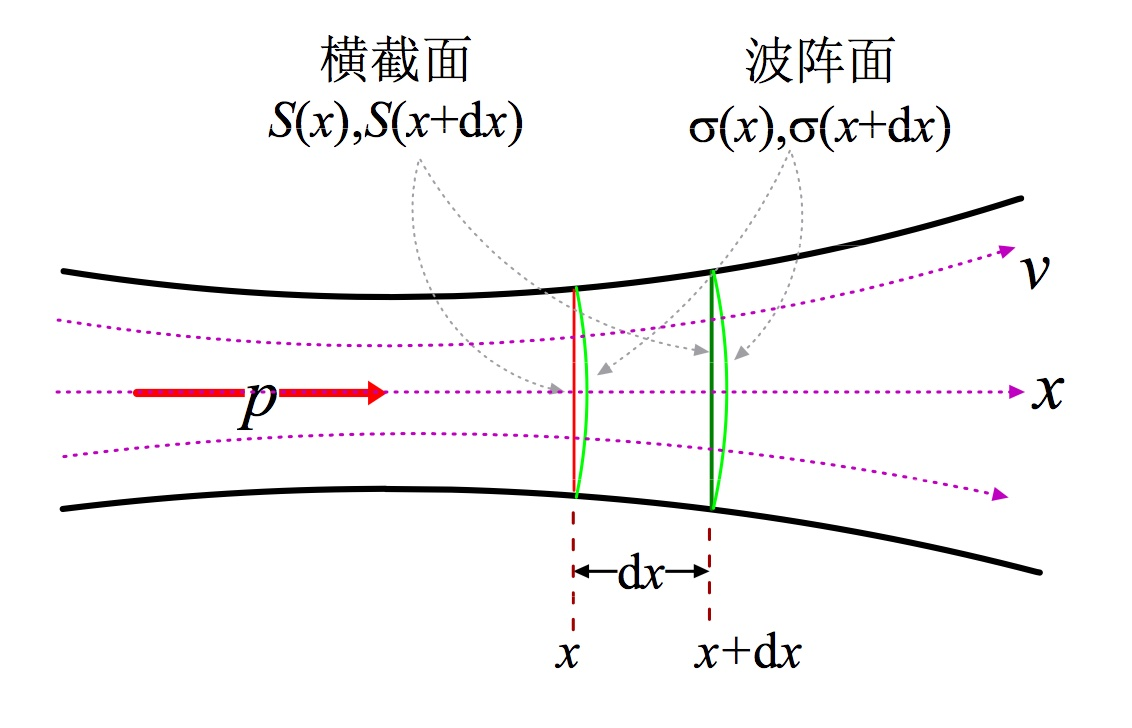
\includegraphics[width=0.7\textwidth]{img/duct/slowlyVaryingPipe.jpg}
	\caption{缓变截面管道模型}
\end{figure}

\subsection{何谓缓变?}
如图(\ref{fig:slowvar_mod})所示的连续变截面管中,管道横截面积和声波波阵面面积皆为管轴向坐标$x$
的函数:
\begin{equation}
	S=S(x)\qc \sigma = \sigma (x)
\end{equation}
因波阵面与管壁正交(壁上法向速度为零),波阵面的面积
$$
\sigma = \iint_\sigma \dd{\sigma} = \iint_\sigma 
\frac{1}{\cos \phi} \dd{S} < \iint_\sigma \frac{1}{\cos\phi_w}\dd{S}
=\frac{S}{\cos\phi_w}$$
其中$\phi$为波阵面法向与管轴的夹角,$\phi_w$为管壁的切角($\phi<\phi_w$)。
于是,
缓变指横截面线度是$x$的缓慢变化的函数,所以
\footnote{如管横截面成圆形,则横截面积的平方正比管半径$R(x)$
	$\tan\phi_w = \dv*{R}{x}$。}
$$
\tan \phi_w \propto \dv{x} \sqrt{S} = O(\eps)
$$
$$\cos \phi_w = \dfrac{1}{\sqrt{1+\tan^2 \phi_w}} = 1+O(\eps^2)
$$
其中$\eps$描述管截面变化的程度。缓变意味着$0<\eps \ll 1$。结果
\begin{equation}
	\label{eq:slowvar_approx}
	\sigma = S\qty[1+O(\eps^2)] \xrightarrow{\ln} \ln \sigma = 
	\ln S+O(\eps^2) \xrightarrow{\dv{x}} \frac1\sigma \dv{\sigma}{x}
	=\frac1S \dv{S}{x}  + O(\eps^2)
\end{equation}

因此,在缓变条件下,$\sigma \approx S$,且$(1/\sigma ) \dv*{\sigma}{x}
\approx (1/S)\dv*{S}{x}$。

\subsection{缓变声管中的声波方程}
回到原坐标$x$,并考察如上图所示由两个相距$\dd{x}$的波阵面所围的小区域$
\Delta V=\sigma \dd{x}$。在此域内对连续性方程作体积分:
$$
0 = \iiint_{\Delta V} \qty[\pdv{\rho}{t} + \div(\rho\vb{v})] \dd{V}
=\iiint_{\Delta V} \pdv{\rho}{t} \dd{V} + \iint_{\Delta V}\div (\rho \vb{v})
\dd{V}
$$

$$
\xrightarrow{\text{apply Gauss's Theorem}} \dv{t} \qty(\dd{x} \int_{\sigma
(x)} \rho \dd{\bm{\sigma}}) + \int_{\sigma (x+\dd{x})} 
\rho \vb{v}\vdot \dd{\bm{\sigma}} - \int_{\sigma(x)} \rho\vb{v} \vdot \dd
\bm{\sigma} = 0
$$

$$
\xrightarrow{\displaystyle f(x+\dd{x})-f(x) = \dv{f}{x} \dd{x}} 
\dv{t} \qty(\iint_{\sigma(x)} \rho \dd{\bm{\sigma}}) \dd{x}
+\pdv{x} \qty(\iint_{\sigma(x)} \rho \vb{v} \vdot \dd{\bm{\sigma}})\dd x
=0
$$

一般认为,运动与状态量(如密度$\rho$)、以及声学量在波阵面$\sigma$上是常数。
因此,上式中的密度$\rho$可从积分号下取出,而得到管内连续性方程的一维形式:
$$
\pdv{\rho}{t} +\frac1\sigma \pdv{x} (\rho U) = 0\qc \qty(U = \iint_\sigma
\vb{v}\vdot \dd{\bm{\sigma}} = v\sigma) = 0$$
其中$U$为经过波阵面的体积流,为横轴坐标$x$的函数。
因波阵面上速度$v$恒常,垂直波阵面法向,故$U=v\sigma$。
管内运动方程和状态方程一如理想流体者。
经小振幅线性化,连续性方程、运动方程和状态方程依次可近似为:
$$
\begin{cases}
	\displaystyle \pdv{\rho'}{t} +\rho_0 \frac1\sigma \pdv{x}(\sigma v) = 0\\[1em]
\displaystyle \rho_0\pdv{v}{t} = -\pdv{p}{x}\\
p = c_0^2 \rho'
\end{cases}
$$
其中$\rho'$为管内密度扰动量,$\rho_0$为静态密度,$p(x)$为声压。
消去$\rho'$和$v$,得一维声压波动方程,
\begin{equation}
	\label{eq:slowvar_sigmawe}
	\frac1\sigma \pdv{x} \qty[\sigma \pdv{p}{x}]
	-\frac{1}{c_0^2} \pdv[2]{p}{t} =0
\end{equation}
然而,与横截面面积$S$不同,波阵面面积$\sigma$难于获得。
为克服困难,把第一项展开,并应用缓变近似(\ref{eq:slowvar_approx}),
$$
\frac{1}{\sigma}\dv{\sigma}{x} \pdv{p}{x}
+\pdv[2]{p}{x} \approx \frac1S \dv{S}{x} \pdv{p}{x}
+\pdv[2]{p}{x} =\frac1S \pdv{x}(S\pdv{p}{x})$$
如此,方程(\ref{eq:slowvar_sigmawe})可近似为
$$
\frac1S \pdv{x} \qty[S\pdv{p}{x}] -\frac{1}{c_0^2}
\pdv[2]{p}{t} = 0
$$
对于频率$\omega$、波数$k$的时间简谐的声波,此方程简化为
\begin{equation}
	\label{eq:slowvar_helmeq}
	\frac1S \pdv{x}\qty(S\pdv{p}{x}) +k^2p = 0
	\qor
	\pdv[2]{p}{x}+\dv{\ln S}{x} \pdv{p}{x}+k^2p=0
\end{equation}
此乃变系数二阶常微分方程\footnote{此方程与密度非均匀媒质的声波方程(一维)
一致,只要互换$1/S$和$\rho$即可。}。

若把$p$当作「位移」,$x$视为「时间」,$k$视为「固有频率」,方程
(\ref{eq:slowvar_helmeq})岂非质点阻尼振动方程?
只不过,此处阻尼系数$\dv*{\ln S}{x}$是「时间」$x$的函数,且可正可负。
若恰好「阻尼系数」为常数,则方程(\ref{eq:slowvar_helmeq})乃常系数二阶常
微分方程,其解当为人所熟知。
此要求横截面$S$按指数形变化。

若$\dv*{\ln S}{x}$非常数,求解方程(\ref{eq:slowvar_helmeq})殊非易事,需借助
适当的数学方法。
对方程(\ref{eq:slowvar_helmeq})作函数变换:
\begin{equation}
	\label{eq:slowvar_ppsi}
	p(x,t) = \frac{\Psi(x,t)}{R(x)}\qc \qty(R=\sqrt{\frac{S}{S_0}})
\end{equation}
其中$S_0$为某参考面积。波函数$\Psi(x,t)$满足二阶常微分方程:
\begin{equation}
	\label{eq:slowvar_psi}
	\pdv[2]{\Psi}{x} +\qty[k^2-u(x)]\Psi=0
\end{equation}
其不含波函数一阶导数项,而变参数$u(x)$定义为
\begin{equation}
	\label{eq:slowvar_u}
	u(x) \equiv \frac{1}{R(x)} \dv[2]{x} R(x)
\end{equation}
它由管横截面$S$确定。反之,若按设计给定$u(x)$,则可以通过以下二阶常微分方程
\begin{equation}
	\dv[2]{R}{x} - u(x)R=0
\end{equation}
反求符合设计要求的横截面$S(x)$。
方程(\ref{eq:slowvar_psi})是标准的Sturm-Liouville型问题,对于诸多形式的
$u(x)$,存在解析解。
在量子力学中它描述电子穿越势垒(势阱)的量子散射问题,$u(x)$是势函数。

\subsection{典型缓变截面管及其声场}
存在$u(x)$恰为常数的特殊情形,数学处理极其简单,无须求助复杂的数学方法。
记
$$u=\mu^2$$
如此,立刻得到方程(\ref{eq:slowvar_psi})的解:
\begin{equation}
	\label{eq:slowvar_psipm}
	\Psi_\pm = \Psi_{\mathrm{a},\pm} \me^{\mj(\omega t\mp \gamma x)}
	\qc \qty(\gamma = \sqrt{k^2-\mu^2})
\end{equation}
其中「$\pm$」表示分别沿管轴正向和反向传播。
此声波解存在\emph{截止频率}:
$$
f\st{cutoff} = \frac{\mu c_0}{2\uppi}
$$
当频率低于此频率时,声波是沿管轴指数衰减(增长)的。
欲使$u$恰为此常数,按(\ref{eq:slowvar_u}),$R$只能取如下形式

\begin{subequations}
	\label{eq:slowvar_R}
	\begin{align}
		R & = 1+\frac{x}{x_0}\\
		R& = R_0 \me^{\pm \mu(x-x_0)} \label{eq:slowvar_Rexp} \\
		R&=a\cosh \mu x +b\sinh \mu x \label{eq:slowvar_Rcat}\\
		R& = a\cos \kappa x + b\sin \kappa x\qc (\mu = \mj \kappa)
	\end{align}
\end{subequations}

\begin{itemize}
	\item 锥形($\mu=0$):式中$x_0$为任意常数,表征号筒的扩展程度。
	\item 指数形($\mu>0$):式中$R_0$表征$x=x_0$处号筒的大小。
	\item 悬链线形($\mu>0$):式中$a$和$b$是任意常数。
	\item 正弦形($\mu$是纯虚数)。
\end{itemize}

前三者分别对应于三种典型的声学号筒(horn):锥形、指数形和悬链线形
\footnote{公式(\ref{eq:slowvar_u})中的$u$也可取负的常数值,所得
的$R$呈余弦或正弦形,不过声学上无多大实用意义,故本文不予考虑。}。
把式(\ref{eq:slowvar_psipm})和式(\ref{eq:slowvar_R})代入式(
\ref{eq:slowvar_ppsi}),获得号筒声压通解,再根据谐波速度与声压的一般关系
$$
v=-\frac{1}{\mj k\rho_0c_0} \dv{p}{x}
$$
可获得速度解。

\subsubsection{指数号筒}
不失一般性,设指数号筒函数(\ref{eq:slowvar_Rexp})中的$x_0=0$。
无限长号筒的正向行波解为
\begin{equation}
	\begin{cases}
		p = p\st{a}\me^{-\mu x+\mj(\omega t \mp \gamma x)}\\
		v = v\st{a} \me^{-\mu x + \mj (\omega t\mp \gamma x)}
	\end{cases}
	\qc 
	\qty(v\st{a} = \frac{p\st{a}}{\rho_0c_0} \me^{-\mj \theta}\qc
	\tan\theta = \frac{\mu}{\gamma})
\end{equation}
号筒任意横截面处的声阻抗
\begin{equation}
	Z\st{a}(x) = \frac{p}{U} = \frac{p}{S(x)v}
	=\frac{\rho_0c_0}{S(x)} \me^{\mj \theta}
\end{equation}
而声阻抗率是常数。辐射声功率
$$
W = \frac12 \Re(p^* U)|_{x=0}
=\frac{1}{2} \Re(Z\st{a}|_{x=0}) |U|_{x=0}^2
=\frac12 \rho_0 c_0 S_0 \cos\theta |v\st{a}|^2
$$
在截止频率处$\theta =\uppi /2$,辐射功率为零\footnote{在截止频率下,$k<\mu$
	声场解为
	$$
	\begin{cases}
		\displaystyle p &\displaystyle =p\st{a} \me^{\displaystyle
			-\mu x - \sqrt{\mu^2-k^2}x+\mj \omega
	t}\\
	\displaystyle v&\displaystyle =-\frac{1}{\mj k\rho_0c_0} \pdv{p}{x}
	=\frac{\mu+ \sqrt{\mu^2-k^2}}{\mj k} \frac{p}{\rho_0c_0}
	\end{cases}
$$
其声阻抗为
$$Z\st{a} = \frac{\rho_0c_0}{S(x)} \frac{\mj k}{\mu +\sqrt{\mu^2-k^2}}
=\frac{\rho_0c_0}{S(x)} \frac{\mj \omega}{\omega\st{cutoff}+\sqrt{\omega\st{cutoff}^2}
-\omega^2}
=\mj \omega M\st{a}
$$
$$
\qty(\displaystyle M\st{a} = \frac{1}{\omega\st{cutoff}+\sqrt{\omega\st{cutoff}^2-\omega^2}}
\frac{\rho_0c_0}{S(x)}\qc 
\omega\st{cutoff}=2\uppi f\st{cutoff})$$
这是一个声质量抗,声质量为$M\st{a}$。
}。
当高于截止频率时,$\cos \theta \approx 1$,辐射功率相近乎大活塞的,效率很高
。


\subsubsection{悬链线号筒}
悬链线号筒取式(\ref{eq:slowvar_Rcat})中的$\cosh$型最为合理自然。
同样设$x_0=0$,无限长悬链线号筒的解为:
\begin{equation}
	\begin{cases}
	p&=p\st{a}\sech \mu x \ \me^{\mj (\omega t-\gamma x)}\\
	\rho_0 c_0 v & = p\st{a} \sech \mu x\ \frac{
	\cosh (\mu x-\mj \theta)}{\cosh \mu x} \me^{\mj(\omega t-\gamma x)}
	\end{cases}
	\qc 
	\qty(\tan \theta = \frac{\mu}{\gamma })
\end{equation}

\begin{equation}
	\frac{p}{v} = \rho_0c_0 \frac{\cosh \mu x}{\cosh (\mu x-\mj \theta)}
	\xrightarrow{x\to 0} \frac{\rho_0c_0}{\cos\theta}
\end{equation}
在喉口($x=0$)处的声阻抗
$$Z\st{a}|_{x=0} = \frac{\rho_0c_0}{S_0\cos\theta}$$
为纯声阻,辐射效率很高。辐射声功率
$$W = \frac12 \Re (p^*U) = \frac{1}{2}\frac{\rho_0c_0S_0}{\cos\theta}
|v\st{a}|^2$$
若喉口振速恒定,则当频率接近截止频率时,辐射功率达无穷大,辐射效率极高。
此特性正与指数号筒相反。


\end{document}
